%%%% Header %%%%%%%%%%%%%%%%%%%%%%%%%%%%%%%%%%%%%%%%%%%%%%%%%%%%%%%%%%%%%%%%%%%

\documentclass[
  12pt
]{scrartcl}

\usepackage{jonas}

\bibliography{/home/jon/lucile/share/hive/sci/refs/refs.bib}
\hyphenation{}

%%%% Meta data %%%%%%%%%%%%%%%%%%%%%%%%%%%%%%%%%%%%%%%%%%%%%%%%%%%%%%%%%%%%%%%%

\usepackage[
  pdfauthor   ={Jonas Schöley},
  pdftitle    ={A Typology of Demographic Time Scales},
  pdfsubject  ={},
  pdfkeywords ={},
  pdfproducer =Latex,
  pdfcreator  =pdflatex
]{hyperref}

\title{A Typology of \\Demographic Time Scales}
\author{Jonas Schöley}

%%%% Titlepage %%%%%%%%%%%%%%%%%%%%%%%%%%%%%%%%%%%%%%%%%%%%%%%%%%%%%%%%%%%%%%%%

\begin{document}

\maketitle

\begin{abstract}
This technical paper describes the six demographic time scales age, period, birth cohort, death cohort, thanatological age and lifespan and their interrelations. It introduces definitions and technical terms necessary for a classification of the scales and their combinations. The aim of this work is to build up to the \enquote{unified model of demographic time} proposed by \cite{Riffe2015}, which unifies all 6 time scales in a single geometrical space.
\end{abstract}

%%%% Text %%%%%%%%%%%%%%%%%%%%%%%%%%%%%%%%%%%%%%%%%%%%%%%%%%%%%%%%%%%%%%%%%%%%%

\begin{description}
  \item[Demographic time scales] are measurements of time used in demography. We differentiate 6 time scales: Age, calender time, birth cohort, death cohort, thanatological age (time until death) and lifespan.
  \item[The Lexis diagram] is a Cartesian plane with calendar time on the abscissa and age on the ordinate. Cohort diagonals show the relation between age and period.
  \item[A temporal plane] is any $xy$ combination of 2 demographic time scales.
  \item[A temporal space] is any $xyz$ combination of 3 demographic time scales.
  \item[Given scales] are demographic time scales which are mapped to the main axis of a temporal plane or a temporal space (age and period in case of the Lexis diagram).
  \item[Derived scales] are demographic time scales which are calculated from the given scales (cohort in case of the Lexis diagram).
  \item[Lexis scales] are the three scales constituting the Lexis diagram: Age, calendar time and cohort.
  \item[Thanatological scales] are scales which take into account the end of life: Death cohort, time until death and lifespan.
  \item[An informative combination] is any combination of given scales which allows for the calculation of derived scales.
  \item[A non-informative combination] is any combination of given scales which does not allow for the calculation of derived scales.
\end{description}

\begin{table}[!htb]
  \small
  \begin{tabularx}{\textwidth}{p{0.23\textwidth}p{0.06\textwidth}XX}
  \toprule
  \textbf{Time Scale} & \textbf{Short} & \textbf{Demographic Defntn.} & \textbf{Event History Defntn.} \\
  \midrule
  Age & $A$ & Time since birth & Time since study entry \\
  Period & $P$ & Calendar time & Calendar time \\
  Birth cohort & $C$ & Calendar time of birth & Calendar time of study entry \\
  Death cohort & $D$ & Calendar time of death & Calendar time of event \\
  Thanatological Age & $T$ & Time until death & Time until event \\
  Lifespan & $L$ & Age at death & Exposure time \\
  \bottomrule
  \end{tabularx}
  \caption{Definitions of various demographic time scales.}
  \label{tab:def}
\end{table}

\clearpage

\begin{center}
  \small
  \begin{longtable}{m{0.1\textwidth}m{0.15\textwidth}m{0.4\textwidth}m{0.17\textwidth}}
  \toprule
  \multicolumn{4}{m{0.9\textwidth}}{\footnotesize\emph{Note:} The temporal planes are named after the two given time scales. The derived scale is appended in parentheses. Contrary to mathematical convention we name the ordinate scale first and the abscissa scale second. This is to be consistent with the established $APC$ and $ACP$ terms.} \\
  \midrule
  %%%%%%%%%%%%%%%%%%%%%%%%%%%%%%%%%%%%%%%%%%%%%%%%%%%%%%%%%%%%%%%%%%%%%%%%%%%%%
  \multicolumn{4}{c}{\textsc{Variations of the Lexis Diagram}} \\
  \midrule
  %%%% AP
  $AP(C)$ & $C = P - A$ &
  The $AP(C)$ temporal plane constitutes the classical Lexis diagram. &
  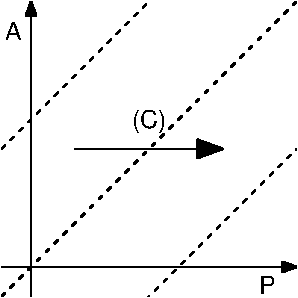
\includegraphics[width = \linewidth]{../fig/APc.pdf} \\
  \midrule
  %%%% AC
  $AC(P)$ & $P = C + A$ &
  The $AC(P)$ temporal plane is equivalent to the Lexis diagram only that birth cohort is given and period is embedded instead of the other way round. &
  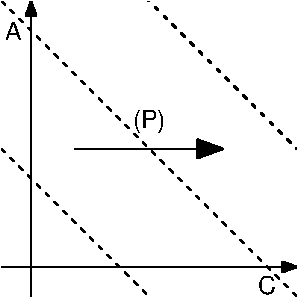
\includegraphics[width = \linewidth]{../fig/ACp.pdf} \\
  \midrule
  %%%% PC
  $CP(A)$ & $A = P - C$ &
  The $CP(A)$ temporal plane is equivalent to the Lexis diagram only that birth cohort is given and age is embedded instead of the other way round. &
  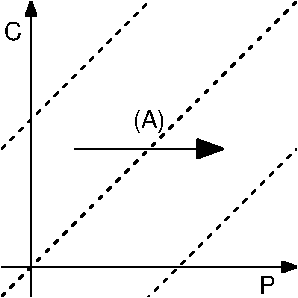
\includegraphics[width = \linewidth]{../fig/CPa.pdf} \\
  \midrule
  %%%%%%%%%%%%%%%%%%%%%%%%%%%%%%%%%%%%%%%%%%%%%%%%%%%%%%%%%%%%%%%%%%%%%%%%%%%%%
  \multicolumn{4}{c}{\textsc{2-D Combinations of Thanatological Scales}} \\
  \midrule
  %%%% LD
  $LD(C)$ & $C = D - L$ & 
  foo. &
  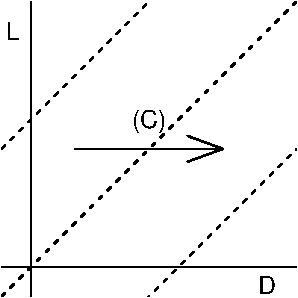
\includegraphics[width = \linewidth]{../fig/LDc.pdf} \\
  \midrule
  %%%% LT
  $TL(A)$ & $A = L - T$ & 
  foo. &
  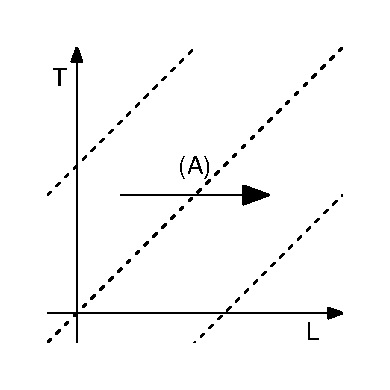
\includegraphics[width = \linewidth]{../fig/TLa.pdf} \\
  \midrule
  %%%% TD
  $TD(P)$ & $P = D - T$ &
  foo. &
  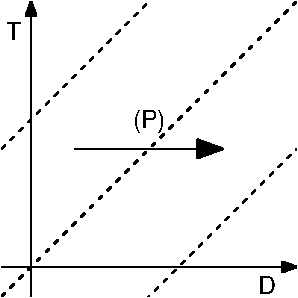
\includegraphics[width = \linewidth]{../fig/TDp.pdf} \\
  \midrule
  %%%%%%%%%%%%%%%%%%%%%%%%%%%%%%%%%%%%%%%%%%%%%%%%%%%%%%%%%%%%%%%%%%%%%%%%%%%%%
  \multicolumn{4}{c}{\textsc{2-D Combinations of Lexis Scales and Thanatological Scales}} \\
  \midrule
  %%%% AL
  $AL(T)$ & $T = A - L$ &
  foo. &
  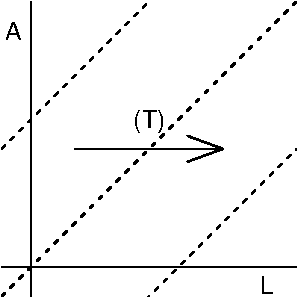
\includegraphics[width = \linewidth]{../fig/ALt.pdf} \\
  \midrule
  %%%% LP
  $LP(-)$ & $-$ &
  The $LP$ plane is \emph{non-informative}. No additional dimensions can be derived knowing just lifespan and period. &
  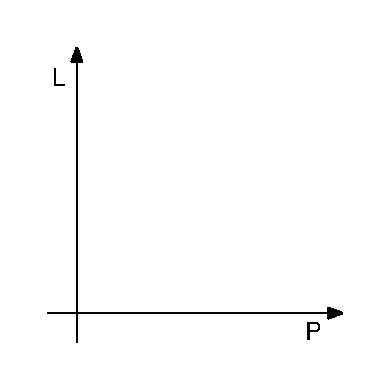
\includegraphics[width = \linewidth]{../fig/LP.pdf} \\
  \midrule
  %%%% PD
  $PD(T)$ & $T = D - P$ &
  foo. &
  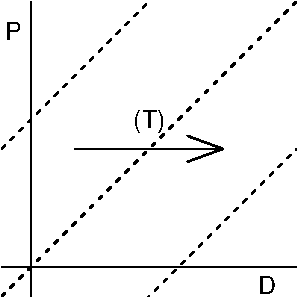
\includegraphics[width = \linewidth]{../fig/PDt.pdf} \\
  \midrule
  %%%% CD
  $CD(L)$ & $L = D - C$ &
  foo. &
  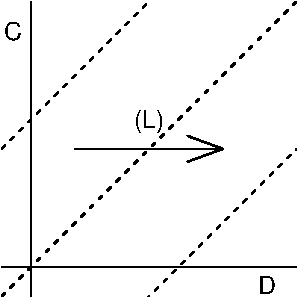
\includegraphics[width = \linewidth]{../fig/CDl.pdf} \\
  \midrule
  %%%% CT
  $CT(-)$ & $-$ &
  The $CT$ plane is \emph{non-informative}. No additional dimensions can be derived knowing just cohort and thanatological age. &
  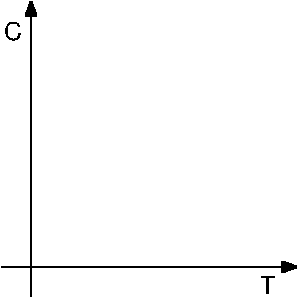
\includegraphics[width = \linewidth]{../fig/CT.pdf} \\
  \midrule
  %%%% TA
  $TA(L)$ & $L = T + A$ &
  The time already lived and the time still left sum up to the total lifespan. &
  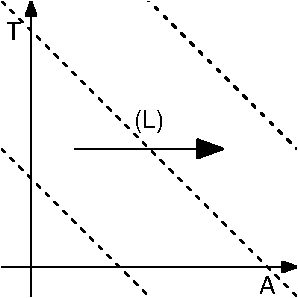
\includegraphics[width = \linewidth]{../fig/TAl.pdf} \\
  \midrule
  %%%% AD
  $AD(-)$ & $-$ &
  The $AD$ plane is \emph{non-informative}. No additional dimensions can be derived knowing just death cohort and age. &
  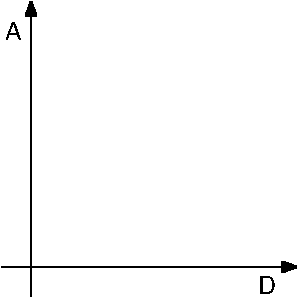
\includegraphics[width = \linewidth]{../fig/AD.pdf} \\
  \midrule
  %%%% LC
  $LC(D)$ & $D = C + L$ &
  foo. &
  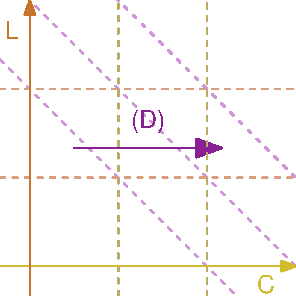
\includegraphics[width = \linewidth]{../fig/LCd.pdf} \\
  \midrule
  %%%% TP
  $TP(-)$ & $-$ &
  The $TP$ plane is \emph{non-informative}. No additional dimensions can be derived knowing just thanatological age and period. &
  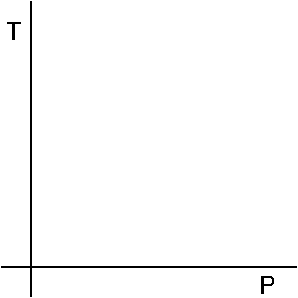
\includegraphics[width = \linewidth]{../fig/TP.pdf} \\
  \bottomrule
  \end{longtable}
  %\caption{Temporal planes: 2-d combinations of demographic time scales.}
  %\label{tab:plane}
\end{center}

\clearpage

%%%% Bibliography %%%%%%%%%%%%%%%%%%%%%%%%%%%%%%%%%%%%%%%%%%%%%%%%%%%%%%%%%%%%%

\sloppy
\printbibliography

%\clearpage

%%%% Appendix %%%%%%%%%%%%%%%%%%%%%%%%%%%%%%%%%%%%%%%%%%%%%%%%%%%%%%%%%%%%%%%%%

% appendix figures follow A1, A2, B1... scheme
%\renewcommand\thefigure{\thesection.\arabic{figure}}
%\setcounter{figure}{0}

%\begin{appendix}
%\end{appendix}

\end{document}